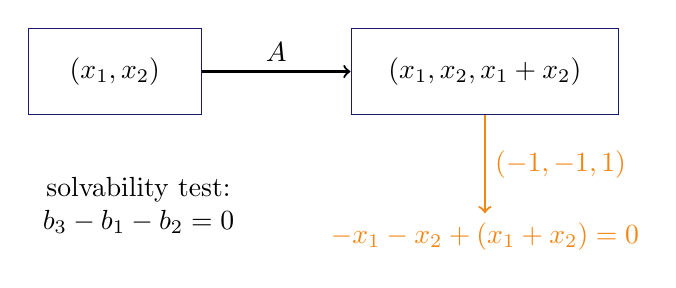
\begin{tikzpicture}[x=1cm,y=1cm]
\node[align=center,draw=MidnightBlue,minimum width=2.2cm,minimum height=1.1cm] (x) at (0,0) {$(x_1,x_2)$};
\node[align=center,draw=MidnightBlue,minimum width=3.4cm,minimum height=1.1cm] (a) at (4.7,0) {$(x_1,x_2,x_1+x_2)$};
\draw[->,thick] (x)--(a) node[midway,above] {$A$};
\draw[->,BurntOrange,thick] (a.south)--(4.7,-1.8) node[midway,right] {$(-1,-1,1)$};
\node[BurntOrange] at (4.7,-2.1) {$-x_1-x_2+(x_1+x_2)=0$};
\node[align=center] at (.3,-1.7) {solvability test:\\$b_3-b_1-b_2=0$};
\end{tikzpicture}
